
% referencias
\addbibresource{./files/gbTeXbib-seminarioUBA.bib}

% glosarios

\newglossaryentry{@glo225-afip}{
type = \acronymtype,
name         = {AFIP},
description  = {Administración Federal de Ingresos Públicos},
first        = {Administración Federal de Ingresos Públicos (AFIP)},
text         = {AFIP},
}
\newglossaryentry{@glo231-teoriadelaediciondelibros}{
name         = {Teoría de la edición de libros:},
description  = {conjunto de principios y enfoques que estudian el proceso de edición de textos, incluyendo la selección, corrección, diseño, producción y difusión de libros. Analiza el papel del editor, la relación con los autores y lectores, así como los factores comerciales, culturales y tecnológicos que influyen en la publicación},
}

\ifPDF
% separata de capítulos solo en pdf de pantalla
\newcounter{PrimPag}
\setcounter{PrimPag}{1}
\setcounter{PrimPag}{\theCurrentPage+1}
\newwrite\script
\immediate\openout\script=separatas.sh
\immediate\write\script{\string#!/bin/bash}
\newcommand{\separata}[1]{\immediate\write\script{pdftk ./pdf/\jobname.pdf cat \thePrimPag-\theCurrentPage\space output ./docs/#1-\jobname.pdf}}

% control de inconsistencias de principio y fin de linea
\usepackage[hyphenation,homeoarchy,homeoarchywordcolor=orange, homeoarchycharcolor=orange,draft]{impnattypo}
\usepackage[allcolors=magenta, colorlinks, unicode]{hyperref}
\usepackage{easyReview}
\usepackage{hyperxmp}

% contenido agregado de manera dinámica, no edite este archivo

\begin{document}
\def\Author{Alberto Moyano}
\def\Title{Lorem Ipsum: Un estudio preliminar sobre las marcas}
\Configure{OpfMetadata}
{\HCode{<dc:subject>Producción editorial, Fuente única, Automatización, Gestión de contenidos, Publicación digital, Formatos múltiples, Distribución eficiente, Edición estructurada, Herramientas colaborativas, Coherencia editorial, Metodología editorial, Optimización del flujo de trabajo, Diseño de publicaciones, Transformación digital, Calidad de contenido.</dc:subject>}}
\Configure{OpfMetadata}
{\HCode{<dc:date>2024-09</dc:date>}}
\Configure{OpfMetadata}
{\HCode{<dc:created></dc:created>}}
\Configure{OpfMetadata}
{\HCode{<dc:modified></dc:modified>}}
\Configure{OpfMetadata}
{\HCode{<dc:rights>Copyright</dc:rights>}}
\Configure{OpfMetadata}
{\HCode{<dc:publisher>Ediciones Imago Mundi</dc:publisher>}}
\Configure{OpfMetadata}
{\HCode{<dc:identifier id="isbn" opf:scheme="ISBN">ISBN:978-950-793-000-0</dc:identifier>}}
\Configure{OpfMetadata}
{\HCode{<dc:identifier id="url" opf:scheme="URL">https://www.edicionesimagomundi.com/</dc:identifier>}}
\Configure{OpfMetadata}
{\HCode{<dc:identifier id="uuid" opf:scheme="uuid">urn:uuid:gbTeXpublisher-03abril2025-00:40:00</dc:identifier>}}
\Configure{DocumentLanguage}{es}
\Configure{OpfMetadata}
{\HCode{<dc:relation>Sin colección</dc:relation>}}
\Configure{OpfMetadata}
{\HCode{<dc:format>EPUB</dc:format>}}
\EndPreamble


	\else
	\ifBNPDF
	\usepackage[width=18truecm,height=25.5truecm,cam,center]{crop}
	\newcommand*\infofont[1]{\sf{\footnotesize #1 (alberto.alejandro.moyano@gmail.com)}}
	\crop[font=infofont]
	\usepackage[hidelinks, unicode]{hyperref}
	\usepackage{hyperxmp}
	
% contenido agregado de manera dinámica, no edite este archivo

\begin{document}
\def\Author{Alberto Moyano}
\def\Title{Lorem Ipsum: Un estudio preliminar sobre las marcas}
\Configure{OpfMetadata}
{\HCode{<dc:subject>Producción editorial, Fuente única, Automatización, Gestión de contenidos, Publicación digital, Formatos múltiples, Distribución eficiente, Edición estructurada, Herramientas colaborativas, Coherencia editorial, Metodología editorial, Optimización del flujo de trabajo, Diseño de publicaciones, Transformación digital, Calidad de contenido.</dc:subject>}}
\Configure{OpfMetadata}
{\HCode{<dc:date>2024-09</dc:date>}}
\Configure{OpfMetadata}
{\HCode{<dc:created></dc:created>}}
\Configure{OpfMetadata}
{\HCode{<dc:modified></dc:modified>}}
\Configure{OpfMetadata}
{\HCode{<dc:rights>Copyright</dc:rights>}}
\Configure{OpfMetadata}
{\HCode{<dc:publisher>Ediciones Imago Mundi</dc:publisher>}}
\Configure{OpfMetadata}
{\HCode{<dc:identifier id="isbn" opf:scheme="ISBN">ISBN:978-950-793-000-0</dc:identifier>}}
\Configure{OpfMetadata}
{\HCode{<dc:identifier id="url" opf:scheme="URL">https://www.edicionesimagomundi.com/</dc:identifier>}}
\Configure{OpfMetadata}
{\HCode{<dc:identifier id="uuid" opf:scheme="uuid">urn:uuid:gbTeXpublisher-03abril2025-00:40:00</dc:identifier>}}
\Configure{DocumentLanguage}{es}
\Configure{OpfMetadata}
{\HCode{<dc:relation>Sin colección</dc:relation>}}
\Configure{OpfMetadata}
{\HCode{<dc:format>EPUB</dc:format>}}
\EndPreamble


		\else
		\ifPNGEPUB
		\usepackage[hidelinks, unicode]{hyperref}
			\else
			\ifHTMLEPUB
			\usepackage[allcolors=blue,colorlinks,hyperindex=true,unicode]{hyperref}
			\fi
		\fi
	\fi
\fi

% Definir el color de fondo: gris con 10% de magenta
\definecolor{chaptercircle}{cmyk}{0,0.1,0,0}

\begin{document}
\frontmatter

\ifHTMLEPUB
	\ifdefined\HCode
	\phantomsection
%	\addcontentsline{toc}{chapter}{Imagen de tapa}
	\coverimage[natwidth=\paperwidth,natheight=\paperheight]{./tapa/cover.png}
	\newpage
	\fi
\fi

\ifPDF
\ifPDF
\PaginaEnBlanco
\PaginaEnBlanco
	\else
	\ifBNPDF
	\PaginaEnBlanco
	\PaginaEnBlanco
	\fi
\fi

% página 3
\newpage
\thispagestyle{empty}
{\textcolor{white}{.}}

\vspace{30mm}

\begin{center}
	\LARGE{Lorem Ipsum}
\end{center}

% página 4
\ifPDF
\PaginaEnBlanco
	\else
	\ifBNPDF
	\PaginaEnBlanco
	\fi
\fi

% página 5
\newpage
\thispagestyle{empty}
\begin{center}%,draft
{\sc\large{alberto moyano}}\\ %compiladoras
\end{center}

\vspace{30mm}

\begin{center}
\LARGE{Lorem Ipsum}\\\vspace{10mm}

\Large{Un estudio preliminar sobre las marcas}
\end{center}

\vfill

\begin{figure}[b]
\centering
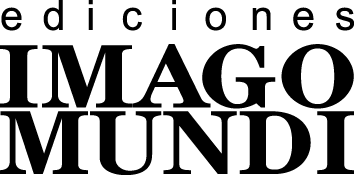
\includegraphics[width=20mm]{./media/logo-imago-ByW.png}
\end{figure}

% página 6
\newpage
\thispagestyle{empty}
\begin{figure}[t]
\centering
\vspace{-10mm}

\includegraphics[width=20mm]{./media/desconocido.png}\\
\end{figure}

\noindent Alberto Moyano \\
\noindent Lorem Ipsum. Un estudio preliminar sobre las marcas. 1\sptext{ra}~ed. Buenos Aires: 2025.\\
\noindent \ztotpages\ p.; \valorEspecifico. ISBN 978-950-793-000-0 \\
\noindent 1. \\
\noindent CDD .\\
\noindent Fecha de catalogación: 21/03/2025 \\
\noindent \textcopyright~2025, Alberto Moyano \\
\noindent \textcopyright~2025, Ediciones Imago Mundi\\
\noindent Imagen de tapa: captura tomada de la web.\\
\noindent Hecho el depósito que marca la ley 11.723\\
\noindent Impreso en Argentina, tirada de esta edición: 000 ejemplares\\

\vfill

\noindent \qrcode[height=2cm]{https://github.com/albertomoyano/seminarioUBA2025}\bigskip

\noindent Ninguna parte de esta publicación, incluido el diseño de cubierta, puede ser reproducida, almacenada o transmitida de manera alguna ni por ningún medio, ya sea eléctrico, químico, mecánico, óptico, de grabación o de fotocopia, sin permiso previo por escrito del editor. Este libro se terminó de imprimir en el mes de marzo de 2025 en San Carlos Impresiones, Virrey Liniers 2203, Ciudad Autónoma de Buenos Aires, República Argentina.

\Author{Sumario}
\tableofcontents
	\else
	\ifBNPDF
	\ifPDF
\PaginaEnBlanco
\PaginaEnBlanco
	\else
	\ifBNPDF
	\PaginaEnBlanco
	\PaginaEnBlanco
	\fi
\fi

% página 3
\newpage
\thispagestyle{empty}
{\textcolor{white}{.}}

\vspace{30mm}

\begin{center}
	\LARGE{Lorem Ipsum}
\end{center}

% página 4
\ifPDF
\PaginaEnBlanco
	\else
	\ifBNPDF
	\PaginaEnBlanco
	\fi
\fi

% página 5
\newpage
\thispagestyle{empty}
\begin{center}%,draft
{\sc\large{alberto moyano}}\\ %compiladoras
\end{center}

\vspace{30mm}

\begin{center}
\LARGE{Lorem Ipsum}\\\vspace{10mm}

\Large{Un estudio preliminar sobre las marcas}
\end{center}

\vfill

\begin{figure}[b]
\centering
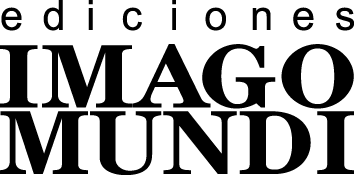
\includegraphics[width=20mm]{./media/logo-imago-ByW.png}
\end{figure}

% página 6
\newpage
\thispagestyle{empty}
\begin{figure}[t]
\centering
\vspace{-10mm}

\includegraphics[width=20mm]{./media/desconocido.png}\\
\end{figure}

\noindent Alberto Moyano \\
\noindent Lorem Ipsum. Un estudio preliminar sobre las marcas. 1\sptext{ra}~ed. Buenos Aires: 2025.\\
\noindent \ztotpages\ p.; \valorEspecifico. ISBN 978-950-793-000-0 \\
\noindent 1. \\
\noindent CDD .\\
\noindent Fecha de catalogación: 21/03/2025 \\
\noindent \textcopyright~2025, Alberto Moyano \\
\noindent \textcopyright~2025, Ediciones Imago Mundi\\
\noindent Imagen de tapa: captura tomada de la web.\\
\noindent Hecho el depósito que marca la ley 11.723\\
\noindent Impreso en Argentina, tirada de esta edición: 000 ejemplares\\

\vfill

\noindent \qrcode[height=2cm]{https://github.com/albertomoyano/seminarioUBA2025}\bigskip

\noindent Ninguna parte de esta publicación, incluido el diseño de cubierta, puede ser reproducida, almacenada o transmitida de manera alguna ni por ningún medio, ya sea eléctrico, químico, mecánico, óptico, de grabación o de fotocopia, sin permiso previo por escrito del editor. Este libro se terminó de imprimir en el mes de marzo de 2025 en San Carlos Impresiones, Virrey Liniers 2203, Ciudad Autónoma de Buenos Aires, República Argentina.

	\Author{Sumario}
	\tableofcontents
		\else
		\ifPNGEPUB
		\ifPDF
\PaginaEnBlanco
\PaginaEnBlanco
	\else
	\ifBNPDF
	\PaginaEnBlanco
	\PaginaEnBlanco
	\fi
\fi

% página 3
\newpage
\thispagestyle{empty}
{\textcolor{white}{.}}

\vspace{30mm}

\begin{center}
	\LARGE{Lorem Ipsum}
\end{center}

% página 4
\ifPDF
\PaginaEnBlanco
	\else
	\ifBNPDF
	\PaginaEnBlanco
	\fi
\fi

% página 5
\newpage
\thispagestyle{empty}
\begin{center}%,draft
{\sc\large{alberto moyano}}\\ %compiladoras
\end{center}

\vspace{30mm}

\begin{center}
\LARGE{Lorem Ipsum}\\\vspace{10mm}

\Large{Un estudio preliminar sobre las marcas}
\end{center}

\vfill

\begin{figure}[b]
\centering
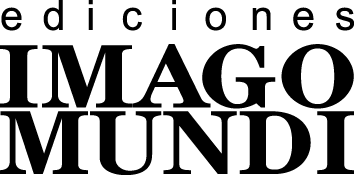
\includegraphics[width=20mm]{./media/logo-imago-ByW.png}
\end{figure}

% página 6
\newpage
\thispagestyle{empty}
\begin{figure}[t]
\centering
\vspace{-10mm}

\includegraphics[width=20mm]{./media/desconocido.png}\\
\end{figure}

\noindent Alberto Moyano \\
\noindent Lorem Ipsum. Un estudio preliminar sobre las marcas. 1\sptext{ra}~ed. Buenos Aires: 2025.\\
\noindent \ztotpages\ p.; \valorEspecifico. ISBN 978-950-793-000-0 \\
\noindent 1. \\
\noindent CDD .\\
\noindent Fecha de catalogación: 21/03/2025 \\
\noindent \textcopyright~2025, Alberto Moyano \\
\noindent \textcopyright~2025, Ediciones Imago Mundi\\
\noindent Imagen de tapa: captura tomada de la web.\\
\noindent Hecho el depósito que marca la ley 11.723\\
\noindent Impreso en Argentina, tirada de esta edición: 000 ejemplares\\

\vfill

\noindent \qrcode[height=2cm]{https://github.com/albertomoyano/seminarioUBA2025}\bigskip

\noindent Ninguna parte de esta publicación, incluido el diseño de cubierta, puede ser reproducida, almacenada o transmitida de manera alguna ni por ningún medio, ya sea eléctrico, químico, mecánico, óptico, de grabación o de fotocopia, sin permiso previo por escrito del editor. Este libro se terminó de imprimir en el mes de marzo de 2025 en San Carlos Impresiones, Virrey Liniers 2203, Ciudad Autónoma de Buenos Aires, República Argentina.

		\Author{Sumario}
		\tableofcontents
		\fi
	\fi
\fi

\ifHTMLEPUB
\tableofcontents
\fi


\chapter[\hspace{1.5pc}Presentación]{Presentación}
\chaptermark{Presentación}
\Author{José María Sebastián}
\setcounter{PrimPag}{\theCurrentPage}

% encabezado para autor
\begin{center}
	\nombreautor{josé maría sebastián}\\
	\vspace{20mm}
\end{center}

Nulla facilisi. Proin eget magna vel purus laoreet tincidunt. Suspendisse aliquet nisl sed erat gravida, id tincidunt arcu vulputate. Phasellus ultricies diam et nulla porttitor, quis venenatis felis luctus.

Maecenas et risus eget justo fermentum convallis. Integer sed lectus sit amet est faucibus egestas. Nam dictum, mauris ut pellentesque varius, odio lacus fringilla arcu, et auctor sem magna sed justo.

Suspendisse potenti. Pellentesque vehicula orci et nunc molestie, ut facilisis velit tincidunt. Vivamus euismod mauris vel diam vestibulum, non scelerisque felis varius. Integer euismod, magna vel pharetra lobortis, erat urna porttitor sapien, at tristique velit arcu ut metus.

Curabitur posuere arcu in felis rhoncus, id laoreet tortor iaculis. Donec hendrerit dolor sed semper ultrices. Fusce congue, lacus a sodales faucibus, neque eros luctus lectus, at maximus turpis lacus at lectus.

\gls{@glo231-teoriadelaediciondelibros}
Quisque id eros vitae purus suscipit facilisis id eget libero. Vestibulum dictum dapibus dui, ut consectetur lectus posuere non. Morbi ut justo ac metus euismod feugiat.

Nulla facilisi. Proin eget magna vel purus laoreet tincidunt. Suspendisse aliquet nisl sed erat gravida, id tincidunt arcu vulputate. Phasellus ultricies diam et nulla porttitor, quis venenatis felis luctus.

Maecenas et risus eget justo fermentum convallis. Integer sed lectus sit amet est faucibus egestas. Nam dictum, mauris ut pellentesque varius, odio lacus fringilla arcu, et auctor sem magna sed justo.

Suspendisse potenti. Pellentesque vehicula orci et nunc molestie, ut facilisis velit tincidunt. Vivamus euismod mauris vel diam vestibulum, non scelerisque felis varius. Integer euismod, magna vel pharetra lobortis, erat urna porttitor sapien, at tristique velit arcu ut metus.

Curabitur posuere arcu in felis rhoncus, id laoreet tortor iaculis. Donec hendrerit dolor sed semper ultrices. Fusce congue, lacus a sodales faucibus, neque eros luctus lectus, at maximus turpis lacus at lectus.

Quisque id eros vitae purus suscipit facilisis id eget libero. Vestibulum dictum dapibus dui, ut consectetur lectus posuere non. Morbi ut justo ac metus euismod feugiat.

Nulla facilisi. Proin eget magna vel purus laoreet tincidunt. Suspendisse aliquet nisl sed erat gravida, id tincidunt arcu vulputate. Phasellus ultricies diam et nulla porttitor, quis venenatis felis luctus.

Maecenas et risus eget justo fermentum convallis. Integer sed lectus sit amet est faucibus egestas. Nam dictum, mauris ut pellentesque varius, odio lacus fringilla arcu, et auctor sem magna sed justo.

Suspendisse potenti. Pellentesque vehicula orci et nunc molestie, ut facilisis velit tincidunt. Vivamus euismod mauris vel diam vestibulum, non scelerisque felis varius. Integer euismod, magna vel pharetra lobortis, erat urna porttitor sapien, at tristique velit arcu ut metus.

Curabitur posuere arcu in felis rhoncus, id laoreet tortor iaculis. Donec hendrerit dolor sed semper ultrices. Fusce congue, lacus a sodales faucibus, neque eros luctus lectus, at maximus turpis lacus at lectus.

Quisque id eros vitae purus suscipit facilisis id eget libero. Vestibulum dictum dapibus dui, ut consectetur lectus posuere non. Morbi ut justo ac metus euismod feugiat.

Nulla facilisi. Proin eget magna vel purus laoreet tincidunt. Suspendisse aliquet nisl sed erat gravida, id tincidunt arcu vulputate. Phasellus ultricies diam et nulla porttitor, quis venenatis felis luctus.

Maecenas et risus eget justo fermentum convallis. Integer sed lectus sit amet est faucibus egestas. Nam dictum, mauris ut pellentesque varius, odio lacus fringilla arcu, et auctor sem magna sed justo.

Suspendisse potenti. Pellentesque vehicula orci et nunc molestie, ut facilisis velit tincidunt. Vivamus euismod mauris vel diam vestibulum, non scelerisque felis varius. Integer euismod, magna vel pharetra lobortis, erat urna porttitor sapien, at tristique velit arcu ut metus.

Curabitur posuere arcu in felis rhoncus, id laoreet tortor iaculis. Donec hendrerit dolor sed semper ultrices. Fusce congue, lacus a sodales faucibus, neque eros luctus lectus, at maximus turpis lacus at lectus.

Quisque id eros vitae purus suscipit facilisis id eget libero. Vestibulum dictum dapibus dui, ut consectetur lectus posuere non. Morbi ut justo ac metus euismod feugiat.

\separata{presentacion}

\chapter[\hspace{1.5pc}Prólogo]{Prólogo}
\Author{Alberto Moyano}
\setcounter{PrimPag}{\theCurrentPage}

Nulla facilisi. Proin eget magna vel purus laoreet tincidunt. Suspendisse aliquet nisl sed erat gravida, id tincidunt arcu vulputate. Phasellus ultricies diam et nulla porttitor, quis venenatis felis luctus.

Maecenas et risus eget justo fermentum convallis. Integer sed lectus sit amet est faucibus egestas. Nam dictum, mauris ut pellentesque varius, odio lacus fringilla arcu, et auctor sem magna sed justo.

Suspendisse potenti. Pellentesque vehicula orci et nunc molestie, ut facilisis velit tincidunt. Vivamus euismod mauris vel diam vestibulum, non scelerisque felis varius. Integer euismod, magna vel pharetra lobortis, erat urna porttitor sapien, at tristique velit arcu ut metus.

Curabitur posuere arcu in felis rhoncus, id laoreet tortor iaculis. Donec hendrerit dolor sed semper ultrices. Fusce congue, lacus a sodales faucibus, neque eros luctus lectus, at maximus turpis lacus at lectus.

Quisque id eros vitae purus suscipit facilisis id eget libero. Vestibulum dictum dapibus dui, ut consectetur lectus posuere non. Morbi ut justo ac metus euismod feugiat.

Nulla facilisi. Proin eget magna vel purus laoreet tincidunt. Suspendisse aliquet nisl sed erat gravida, id tincidunt arcu vulputate. Phasellus ultricies diam et nulla porttitor, quis venenatis felis luctus.

Maecenas et risus eget justo fermentum convallis. Integer sed lectus sit amet est faucibus egestas. Nam dictum, mauris ut pellentesque varius, odio lacus fringilla arcu, et auctor sem magna sed justo.

Suspendisse potenti. Pellentesque vehicula orci et nunc molestie, ut facilisis velit tincidunt. Vivamus euismod mauris vel diam vestibulum, non scelerisque felis varius. Integer euismod, magna vel pharetra lobortis, erat urna porttitor sapien, at tristique velit arcu ut metus.

Curabitur posuere arcu in felis rhoncus, id laoreet tortor iaculis. Donec hendrerit dolor sed semper ultrices. Fusce congue, lacus a sodales faucibus, neque eros luctus lectus, at maximus turpis lacus at lectus.

Quisque id eros vitae purus suscipit facilisis id eget libero. Vestibulum dictum dapibus dui, ut consectetur lectus posuere non. Morbi ut justo ac metus euismod feugiat.

Nulla facilisi. Proin eget magna vel purus laoreet tincidunt. Suspendisse aliquet nisl sed erat gravida, id tincidunt arcu vulputate. Phasellus ultricies diam et nulla porttitor, quis venenatis felis luctus.

Maecenas et risus eget justo fermentum convallis. Integer sed lectus sit amet est faucibus egestas. Nam dictum, mauris ut pellentesque varius, odio lacus fringilla arcu, et auctor sem magna sed justo.

Suspendisse potenti. Pellentesque vehicula orci et nunc molestie, ut facilisis velit tincidunt. Vivamus euismod mauris vel diam vestibulum, non scelerisque felis varius. Integer euismod, magna vel pharetra lobortis, erat urna porttitor sapien, at tristique velit arcu ut metus.

Curabitur posuere arcu in felis rhoncus, id laoreet tortor iaculis. Donec hendrerit dolor sed semper ultrices. Fusce congue, lacus a sodales faucibus, neque eros luctus lectus, at maximus turpis lacus at lectus.

Quisque id eros vitae purus suscipit facilisis id eget libero. Vestibulum dictum dapibus dui, ut consectetur lectus posuere non. Morbi ut justo ac metus euismod feugiat.

Nulla facilisi. Proin eget magna vel purus laoreet tincidunt. Suspendisse aliquet nisl sed erat gravida, id tincidunt arcu vulputate. Phasellus ultricies diam et nulla porttitor, quis venenatis felis luctus.

Maecenas et risus eget justo fermentum convallis. Integer sed lectus sit amet est faucibus egestas. Nam dictum, mauris ut pellentesque varius, odio lacus fringilla arcu, et auctor sem magna sed justo.

Suspendisse potenti. Pellentesque vehicula orci et nunc molestie, ut facilisis velit tincidunt. Vivamus euismod mauris vel diam vestibulum, non scelerisque felis varius. Integer euismod, magna vel pharetra lobortis, erat urna porttitor sapien, at tristique velit arcu ut metus.

Curabitur posuere arcu in felis rhoncus, id laoreet tortor iaculis. Donec hendrerit dolor sed semper ultrices. Fusce congue, lacus a sodales faucibus, neque eros luctus lectus, at maximus turpis lacus at lectus.

Quisque id eros vitae purus suscipit facilisis id eget libero. Vestibulum dictum dapibus dui, ut consectetur lectus posuere non. Morbi ut justo ac metus euismod feugiat.

\separata{prologo}
\chapter[\hspace{1.5pc}Introducción]{Introducción}
\chaptermark{Introducción}
\Author{Alberto Moyano}
\setcounter{PrimPag}{\theCurrentPage}

Nulla facilisi. Proin eget magna vel purus laoreet tincidunt. Suspendisse aliquet nisl sed erat gravida, id tincidunt arcu vulputate. Phasellus ultricies diam et nulla porttitor, quis venenatis felis luctus.

Maecenas et risus eget justo fermentum convallis. Integer sed lectus sit amet est faucibus egestas. Nam dictum, mauris ut pellentesque varius, odio lacus fringilla arcu, et auctor sem magna sed justo.

Suspendisse potenti. Pellentesque vehicula orci et nunc molestie, ut facilisis velit tincidunt. Vivamus euismod mauris vel diam vestibulum, non scelerisque felis varius. Integer euismod, magna vel pharetra lobortis, erat urna porttitor sapien, at tristique velit arcu ut metus.

Curabitur posuere arcu in felis rhoncus, id laoreet tortor iaculis. Donec hendrerit dolor sed semper ultrices. Fusce congue, lacus a sodales faucibus, neque eros luctus lectus, at maximus turpis lacus at lectus.

Quisque id eros vitae purus suscipit facilisis id eget libero. Vestibulum dictum dapibus dui, ut consectetur lectus posuere non. Morbi ut justo ac metus euismod feugiat.

Nulla facilisi. Proin eget magna vel purus laoreet tincidunt. Suspendisse aliquet nisl sed erat gravida, id tincidunt arcu vulputate. Phasellus ultricies diam et nulla porttitor, quis venenatis felis luctus.

Maecenas et risus eget justo fermentum convallis. Integer sed lectus sit amet est faucibus egestas. Nam dictum, mauris ut pellentesque varius, odio lacus fringilla arcu, et auctor sem magna sed justo.

Suspendisse potenti. Pellentesque vehicula orci et nunc molestie, ut facilisis velit tincidunt. Vivamus euismod mauris vel diam vestibulum, non scelerisque felis varius. Integer euismod, magna vel pharetra lobortis, erat urna porttitor sapien, at tristique velit arcu ut metus.

Curabitur posuere arcu in felis rhoncus, id laoreet tortor iaculis. Donec hendrerit dolor sed semper ultrices. Fusce congue, lacus a sodales faucibus, neque eros luctus lectus, at maximus turpis lacus at lectus.

Quisque id eros vitae purus suscipit facilisis id eget libero. Vestibulum dictum dapibus dui, ut consectetur lectus posuere non. Morbi ut justo ac metus euismod feugiat.

Nulla facilisi. Proin eget magna vel purus laoreet tincidunt. Suspendisse aliquet nisl sed erat gravida, id tincidunt arcu vulputate. Phasellus ultricies diam et nulla porttitor, quis venenatis felis luctus.

Maecenas et risus eget justo fermentum convallis. Integer sed lectus sit amet est faucibus egestas. Nam dictum, mauris ut pellentesque varius, odio lacus fringilla arcu, et auctor sem magna sed justo.

Suspendisse potenti. Pellentesque vehicula orci et nunc molestie, ut facilisis velit tincidunt. Vivamus euismod mauris vel diam vestibulum, non scelerisque felis varius. Integer euismod, magna vel pharetra lobortis, erat urna porttitor sapien, at tristique velit arcu ut metus.

Curabitur posuere arcu in felis rhoncus, id laoreet tortor iaculis. Donec hendrerit dolor sed semper ultrices. Fusce congue, lacus a sodales faucibus, neque eros luctus lectus, at maximus turpis lacus at lectus.

Quisque id eros vitae purus suscipit facilisis id eget libero. Vestibulum dictum dapibus dui, ut consectetur lectus posuere non. Morbi ut justo ac metus euismod feugiat.

Nulla facilisi. Proin eget magna vel purus laoreet tincidunt. Suspendisse aliquet nisl sed erat gravida, id tincidunt arcu vulputate. Phasellus ultricies diam et nulla porttitor, quis venenatis felis luctus.

Maecenas et risus eget justo fermentum convallis. Integer sed lectus sit amet est faucibus egestas. Nam dictum, mauris ut pellentesque varius, odio lacus fringilla arcu, et auctor sem magna sed justo.

Suspendisse potenti. Pellentesque vehicula orci et nunc molestie, ut facilisis velit tincidunt. Vivamus euismod mauris vel diam vestibulum, non scelerisque felis varius. Integer euismod, magna vel pharetra lobortis, erat urna porttitor sapien, at tristique velit arcu ut metus.

Curabitur posuere arcu in felis rhoncus, id laoreet tortor iaculis. Donec hendrerit dolor sed semper ultrices. Fusce congue, lacus a sodales faucibus, neque eros luctus lectus, at maximus turpis lacus at lectus.

Quisque id eros vitae purus suscipit facilisis id eget libero. Vestibulum dictum dapibus dui, ut consectetur lectus posuere non. Morbi ut justo ac metus euismod feugiat.

Finalmente, Camilo Vicente Ovalle \rdm{de la Universidad Nacional Autónoma de México} introduce el estudio del caso mexicano, un país que no tuvo gobiernos dictatoriales como el resto de los países analizados, aunque colaboró ampliamente en los procesos represivos del área. El trabajo analiza las prácticas de vigilancia y represión del gobierno mexicano en particular dirigidas hacia activistas y organizaciones revolucionarias guatemaltecas \rdm{lo que el autor denomina diplomacia contrainsurgente} expresadas en el intercambio de información, control y desarticulación de redes de apoyo a la guerrilla del país vecino y en la participación en espacios multilaterales coordinados por los Estados Unidos, donde también acudieron militares sudamericanos.

\separata{introduccion}


\mainmatter

\chapter{Lorem Ipsum Dolor Sit Amet}
\Author{Alberto Moyano}
\setcounter{PrimPag}{\theCurrentPage}

\section{Introducción al Lorem Ipsum}

Lorem ipsum dolor sit amet, consectetur adipiscing elit. Quisque sodales, lacus id pellentesque placerat, justo eros laoreet urna, a eleifend libero purus non lacus. Integer feugiat, nisl sit amet varius consequat, sapien dui maximus erat, at eleifend risus eros et velit. Suspendisse vehicula, mauris id euismod interdum, purus est accumsan justo, eget facilisis quam nisi non lacus.\footnote{Para más detalles, véase cuadro~\ref{cap3-1}, en pág.~\pageref{cap3-1}.}

Sed a lorem ac velit accumsan aliquet. Nunc ac erat nec est tincidunt bibendum. Aliquam sagittis fermentum dui, ac gravida lorem faucibus eget. Phasellus id magna id nunc dapibus facilisis.

Lorem ipsum dolor sit amet, consectetur adipiscing elit. Quisque sodales, lacus id pellentesque placerat, justo eros laoreet urna, a eleifend libero purus non lacus. Integer feugiat, nisl sit amet varius consequat, sapien dui maximus erat, at eleifend risus eros et velit. Suspendisse vehicula, mauris id euismod interdum, purus est accumsan justo, eget facilisis quam nisi non lacus.

Sed a lorem ac velit accumsan aliquet. Nunc ac erat nec est tincidunt bibendum. Aliquam sagittis fermentum dui, ac gravida lorem faucibus eget. Phasellus id magna id nunc dapibus facilisis.

\section{Historia y evolución}

Duis vitae purus in lacus interdum dapibus. Nullam tincidunt, augue non feugiat posuere, est erat pharetra tortor, ac molestie quam ligula vel est. Donec id arcu in odio faucibus tincidunt. Phasellus condimentum, lectus ac fermentum tincidunt, mi sapien venenatis justo, id consectetur neque risus in sapien.

Duis vitae purus in lacus interdum dapibus. Nullam tincidunt, augue non feugiat posuere, est erat pharetra tortor, ac molestie quam ligula vel est. Donec id arcu in odio faucibus tincidunt. Phasellus condimentum, lectus ac fermentum tincidunt, mi sapien venenatis justo, id consectetur neque risus in sapien.

Duis vitae purus in lacus interdum dapibus. Nullam tincidunt, augue non feugiat posuere, est erat pharetra tortor, ac molestie quam ligula vel est. Donec id arcu in odio faucibus tincidunt. Phasellus condimentum, lectus ac fermentum tincidunt, mi sapien venenatis justo, id consectetur neque risus in sapien.

\subsection{Uso en la tipografía}

Maecenas sodales mi vel risus vehicula, non ultricies lorem iaculis. Nulla facilisi. Ut congue odio justo, at dapibus velit tincidunt id. Vivamus eget orci vitae urna aliquet dapibus sed sed eros. Integer gravida lacus id justo lacinia, ut faucibus lorem posuere. Curabitur sit amet erat eget nunc ultricies dignissim (véase figura~\ref{figura1-1}).

Maecenas sodales mi vel risus vehicula, non ultricies lorem iaculis. Nulla facilisi. Ut congue odio justo, at dapibus velit tincidunt id. Vivamus eget orci vitae urna aliquet dapibus sed sed eros. Integer gravida lacus id justo lacinia, ut faucibus lorem posuere. Curabitur sit amet erat eget nunc ultricies dignissim.

\ifPDF
\begin{figure}[!ht]
\centering

\includegraphics[width=\textwidth]{./media/letraA.png}
\caption{Variaciones en la letra a. Fuente: tipografía Minion Pro.}\label{figura1-1}
\end{figure}
\else
\ifBNPDF
\begin{figure}[!ht]
	\centering
	
\includegraphics[width=\textwidth]{./media/letraa.png}
	\caption{Variaciones en la letra a. Fuente: tipografía Minion Pro.}\label{figura1-1}
	\end{figure}
	\fi
		\else
		\ifPNGEPUB
		\begin{figure}[!ht]
		\centering
		
\includegraphics[width=\textwidth]{./media/letraa.png}
		\caption{Variaciones en la letra a. Fuente: tipografía Minion Pro.}\label{figura1-1}
		\end{figure}
		\fi
\fi

Maecenas sodales mi vel risus vehicula, non ultricies lorem iaculis. Nulla facilisi. Ut congue odio justo, at dapibus velit tincidunt id. Vivamus eget orci vitae urna aliquet dapibus sed sed eros. Integer gravida lacus id justo lacinia, ut faucibus lorem posuere. Curabitur sit amet erat eget nunc ultricies dignissim.

Maecenas sodales mi vel risus vehicula, non ultricies lorem iaculis. Nulla facilisi. Ut congue odio justo, at dapibus velit tincidunt id. Vivamus eget orci vitae urna aliquet dapibus sed sed eros. Integer gravida lacus id justo lacinia, ut faucibus lorem posuere. Curabitur sit amet erat eget nunc ultricies dignissim.

\section{Aplicaciones modernas}

Pellentesque habitant morbi tristique senectus et netus et malesuada fames ac turpis egestas. Duis in gravida eros, at scelerisque purus. Fusce dignissim, magna vel tincidunt cursus, nisi augue viverra metus, ac posuere augue urna nec eros. Sed efficitur risus vel mi suscipit, et suscipit lorem cursus. Vestibulum in felis quis mauris varius dictum nec a risus \parencite{@6282-DIAMAND1984}.

Etiam elementum suscipit orci, nec vehicula odio pharetra sit amet. Phasellus facilisis ligula ac est hendrerit, id bibendum dui lobortis. In scelerisque libero a dui interdum, ac fermentum odio feugiat.

Pellentesque habitant morbi tristique senectus et netus et malesuada fames ac turpis egestas. Duis in gravida eros, at scelerisque purus. Fusce dignissim, magna vel tincidunt cursus, nisi augue viverra metus, ac posuere augue urna nec eros. Sed efficitur risus vel mi suscipit, et suscipit lorem cursus. Vestibulum in felis quis mauris varius dictum nec a risus.

Etiam elementum suscipit orci, nec vehicula odio pharetra sit amet. Phasellus facilisis ligula ac est hendrerit, id bibendum dui lobortis. In scelerisque libero a dui interdum, ac fermentum odio feugiat.

\section{Conclusiones}

Pellentesque habitant morbi tristique senectus et netus et malesuada fames ac turpis egestas. Duis in gravida eros, at scelerisque purus. Fusce dignissim, magna vel tincidunt cursus, nisi augue viverra metus, ac posuere augue urna nec eros. Sed efficitur risus vel mi suscipit, et suscipit lorem cursus. Vestibulum in felis quis mauris varius dictum nec a risus.

Etiam elementum suscipit orci, nec vehicula odio pharetra sit amet. Phasellus facilisis ligula ac est hendrerit, id bibendum dui lobortis. In scelerisque libero a dui interdum, ac fermentum odio feugiat.

\separata{capitulo1}
\chapter{Consectetur Adipiscing Elit}

\section{La Estructura del texto simulado}

Vestibulum ante ipsum primis in faucibus orci luctus et ultrices posuere cubilia curae; Duis dapibus, nunc nec fermentum malesuada, arcu elit ullamcorper nisi, eget luctus neque erat in elit. Nullam porttitor, nisi vel ultricies consequat, arcu felis tincidunt dolor, ac sagittis ipsum nulla eu eros.

Phasellus vel lacus ut neque rhoncus suscipit. Nam eget mi ut sapien volutpat tincidunt. Donec molestie turpis in eros elementum, et tempor ligula condimentum. Pellentesque habitant morbi tristique senectus et netus et malesuada fames ac turpis egestas.

Vestibulum ante ipsum primis in faucibus orci luctus et ultrices posuere cubilia curae; Duis dapibus, nunc nec fermentum malesuada, arcu elit ullamcorper nisi, eget luctus neque erat in elit. Nullam porttitor, nisi vel ultricies consequat, arcu felis tincidunt dolor, ac sagittis ipsum nulla eu eros.

Phasellus vel lacus ut neque rhoncus suscipit. Nam eget mi ut sapien volutpat tincidunt. Donec molestie turpis in eros elementum, et tempor ligula condimentum. Pellentesque habitant morbi tristique senectus et netus et malesuada fames ac turpis egestas.

Vestibulum ante ipsum primis in faucibus orci luctus et ultrices posuere cubilia curae; Duis dapibus, nunc nec fermentum malesuada, arcu elit ullamcorper nisi, eget luctus neque erat in elit. Nullam porttitor, nisi vel ultricies consequat, arcu felis tincidunt dolor, ac sagittis ipsum nulla eu eros.

Phasellus vel lacus ut neque rhoncus suscipit. Nam eget mi ut sapien volutpat tincidunt. Donec molestie turpis in eros elementum, et tempor ligula condimentum. Pellentesque habitant morbi tristique senectus et netus et malesuada fames ac turpis egestas.

Vestibulum ante ipsum primis in faucibus orci luctus et ultrices posuere cubilia curae; Duis dapibus, nunc nec fermentum malesuada, arcu elit ullamcorper nisi, eget luctus neque erat in elit. Nullam porttitor, nisi vel ultricies consequat, arcu felis tincidunt dolor, ac sagittis ipsum nulla eu eros.

Phasellus vel lacus ut neque rhoncus suscipit. Nam eget mi ut sapien volutpat tincidunt. Donec molestie turpis in eros elementum, et tempor ligula condimentum. Pellentesque habitant morbi tristique senectus et netus et malesuada fames ac turpis egestas.

\section{Variaciones y uso en diseño}

Donec at lacus vitae eros pharetra efficitur. Suspendisse potenti. Morbi tincidunt, libero eget sagittis tempus, ligula justo iaculis erat, vitae tincidunt lectus purus et ligula. Integer eget dolor sed nunc tincidunt sodales.

Ut nec augue vel mauris ultricies interdum. Phasellus venenatis, sapien ut pellentesque facilisis, purus eros bibendum nisl, vitae dictum sem lectus et libero. Nulla auctor, metus vel varius faucibus, urna quam sodales turpis, nec convallis odio justo nec felis.

\subsection{Aplicaciones en la industria editorial}

Praesent sagittis, nisl sed auctor rhoncus, turpis massa fermentum justo, at convallis lorem risus et lorem. Sed id eros nec odio faucibus auctor. Aliquam erat volutpat. Proin vitae quam at ligula ultrices fringilla. Mauris tincidunt velit sed sem dictum, id hendrerit libero laoreet.

Praesent sagittis, nisl sed auctor rhoncus, turpis massa fermentum justo, at convallis lorem risus et lorem. Sed id eros nec odio faucibus auctor. Aliquam erat volutpat. Proin vitae quam at ligula ultrices fringilla. Mauris tincidunt velit sed sem dictum, id hendrerit libero laoreet.

Praesent sagittis, nisl sed auctor rhoncus, turpis massa fermentum justo, at convallis lorem risus et lorem. Sed id eros nec odio faucibus auctor. Aliquam erat volutpat. Proin vitae quam at ligula ultrices fringilla. Mauris tincidunt velit sed sem dictum, id hendrerit libero laoreet.

Praesent sagittis, nisl sed auctor rhoncus, turpis massa fermentum justo, at convallis lorem risus et lorem. Sed id eros nec odio faucibus auctor. Aliquam erat volutpat. Proin vitae quam at ligula ultrices fringilla. Mauris tincidunt velit sed sem dictum, id hendrerit libero laoreet.

\section{Conclusiones}

Nunc malesuada feugiat risus, a pellentesque libero tincidunt ut. Ut eget metus id quam posuere accumsan at vel lacus. Integer imperdiet ex ut ligula lobortis, id elementum risus consectetur. Suspendisse at lectus sed justo pellentesque aliquet.

Curabitur ut massa et metus blandit tincidunt. Fusce convallis fringilla diam, sed suscipit ex dapibus vel. Nam vel nisl nunc. Morbi feugiat mauris sed venenatis tincidunt. Donec at arcu nec quam facilisis interdum ut eget felis.

Nunc malesuada feugiat risus, a pellentesque libero tincidunt ut. Ut eget metus id quam posuere accumsan at vel lacus. Integer imperdiet ex ut ligula lobortis, id elementum risus consectetur. Suspendisse at lectus sed justo pellentesque aliquet.

Curabitur ut massa et metus blandit tincidunt. Fusce convallis fringilla diam, sed suscipit ex dapibus vel. Nam vel nisl nunc. Morbi feugiat mauris sed venenatis tincidunt. Donec at arcu nec quam facilisis interdum ut eget felis.


\chapter{Vestibulum Eget Nisi}
\setcounter{PrimPag}{\theCurrentPage}

\section{Origen y evolución}

Vestibulum eget nisi at erat eleifend malesuada. Curabitur dignissim, tortor at sodales accumsan, nisl odio interdum purus, sed cursus nulla lorem sit amet purus. Integer ac justo vel risus consequat ultrices.

Nam scelerisque velit eget nibh tempus, eget fermentum sapien condimentum. Donec vehicula dapibus tincidunt. Suspendisse vel dictum mi. Etiam sed urna ac risus volutpat fermentum a vel mauris. Aliquam in urna enim.

Vestibulum eget nisi at erat eleifend malesuada. Curabitur dignissim, tortor at sodales accumsan, nisl odio interdum purus, sed cursus nulla lorem sit amet purus. Integer ac justo vel risus consequat ultrices.

Nam scelerisque velit eget nibh tempus, eget fermentum sapien condimentum. Donec vehicula dapibus tincidunt. Suspendisse vel dictum mi. Etiam sed urna ac risus volutpat fermentum a vel mauris. Aliquam in urna enim.

Vestibulum eget nisi at erat eleifend malesuada. Curabitur dignissim, tortor at sodales accumsan, nisl odio interdum purus, sed cursus nulla lorem sit amet purus. Integer ac justo vel risus consequat ultrices.

Nam scelerisque velit eget nibh tempus, eget fermentum sapien condimentum. Donec vehicula dapibus tincidunt. Suspendisse vel dictum mi. Etiam sed urna ac risus volutpat fermentum a vel mauris. Aliquam in urna enim.

\section{Aplicaciones y relevancia en la tipografía}

Aliquam auctor lectus non arcu fermentum, at bibendum tortor luctus. In hac habitasse platea dictumst. Aenean non magna vel est dictum tincidunt. Mauris rhoncus convallis mi, ac suscipit libero interdum a.\footnote{Para más detalles véase la figura~\ref{figura1-1} (pág.~\pageref{figura1-1} en este volumen).}

Sed vehicula, felis sed sodales euismod, ligula mi ullamcorper nisl, sed dictum mauris metus at felis. Nulla facilisi. Pellentesque ut lorem quis nunc gravida molestie at ut nunc. Duis efficitur velit nec leo efficitur, sed laoreet tortor vehicula.

Aliquam auctor lectus non arcu fermentum, at bibendum tortor luctus. In hac habitasse platea dictumst. Aenean non magna vel est dictum tincidunt. Mauris rhoncus convallis mi, ac suscipit libero interdum a.

Sed vehicula, felis sed sodales euismod, ligula mi ullamcorper nisl, sed dictum mauris metus at felis. Nulla facilisi. Pellentesque ut lorem quis nunc gravida molestie at ut nunc. Duis efficitur velit nec leo efficitur, sed laoreet tortor vehicula.

Aliquam auctor lectus non arcu fermentum, at bibendum tortor luctus. In hac habitasse platea dictumst. Aenean non magna vel est dictum tincidunt. Mauris rhoncus convallis mi, ac suscipit libero interdum a.

Sed vehicula, felis sed sodales euismod, ligula mi ullamcorper nisl, sed dictum mauris metus at felis. Nulla facilisi. Pellentesque ut lorem quis nunc gravida molestie at ut nunc. Duis efficitur velit nec leo efficitur, sed laoreet tortor vehicula.

\section{El impacto en la industria}

Curabitur sodales lacus at lorem auctor, sed consectetur sapien feugiat. Fusce dapibus, velit eget iaculis bibendum, lorem nisi efficitur erat, ac ultricies nunc neque ut massa. Proin euismod odio nec nisl eleifend fermentum.

Curabitur sodales lacus at lorem auctor, sed consectetur sapien feugiat. Fusce dapibus, velit eget iaculis bibendum, lorem nisi efficitur erat, ac ultricies nunc neque ut massa. Proin euismod odio nec nisl eleifend fermentum.

Curabitur sodales lacus at lorem auctor, sed consectetur sapien feugiat. Fusce dapibus, velit eget iaculis bibendum, lorem nisi efficitur erat, ac ultricies nunc neque ut massa. Proin euismod odio nec nisl eleifend fermentum.\footnote{Véase cuadro~\ref{cuadro2-1} (pág.~\pageref{cuadro2-1} en este volumen).}

\ifPDF
\begin{figure}[!ht]
	\centering
	
\includegraphics[width=.5\textwidth]{./media/avatar.png}
	\caption{Totoro nos recuerda que la magia está en los detalles \parencite{@6404-HAYAO2005}.}\label{figura3-1}
\end{figure}
\else
\ifBNPDF
\begin{figure}[!ht]
	\centering
	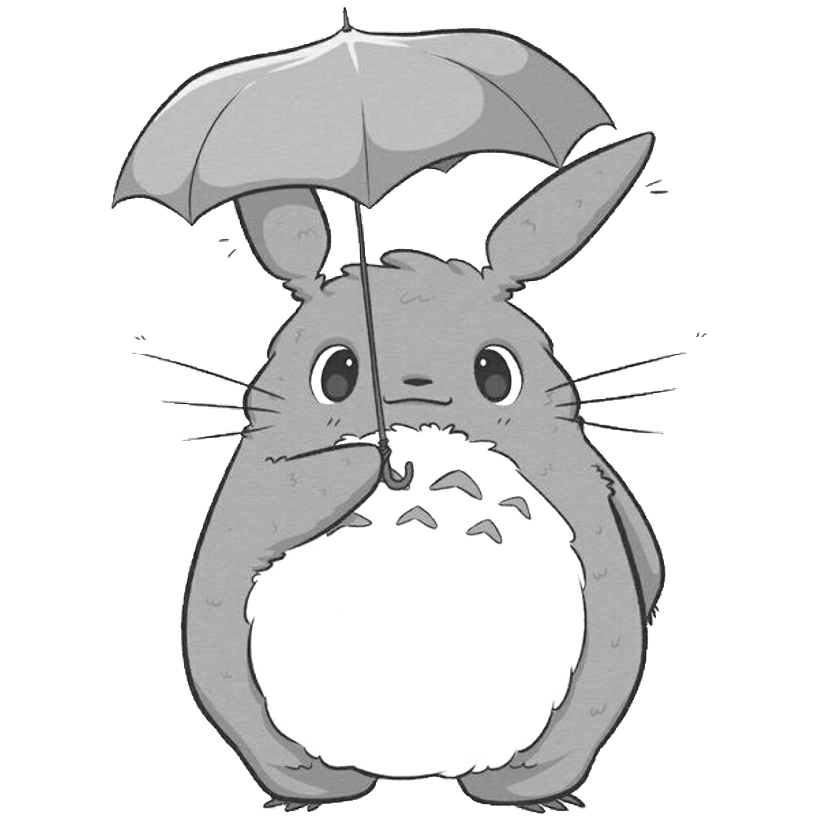
\includegraphics[width=.5\textwidth]{./media/avatar2.png}
	\caption{Totoro nos recuerda que la magia está en los detalles \parencite{@6404-HAYAO2005}.}\label{figura3-1}
\end{figure}
\fi
\else
\ifPNGEPUB
\begin{figure}[!ht]
	\centering
	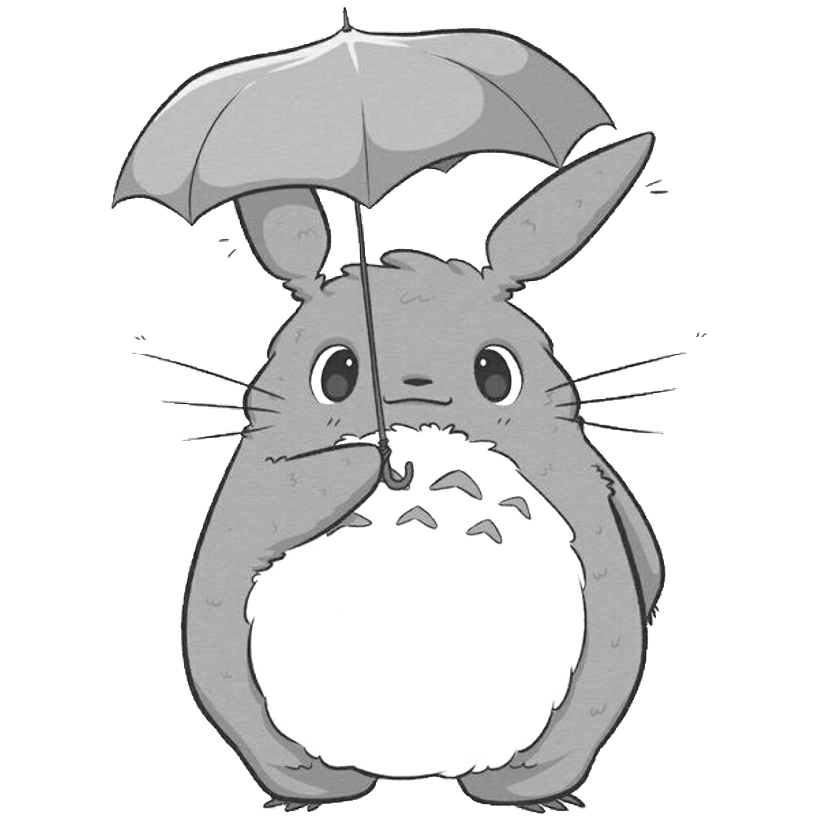
\includegraphics[width=.5\textwidth]{./media/avatar2.png}
	\caption{Totoro nos recuerda que la magia está en los detalles \parencite{@6404-HAYAO2005}.}\label{figura3-1}
\end{figure}
\fi
\fi

Curabitur sodales lacus at lorem auctor, sed consectetur sapien feugiat. Fusce dapibus, velit eget iaculis bibendum, lorem nisi efficitur erat, ac ultricies nunc neque ut massa. Proin euismod odio nec nisl eleifend fermentum.

Curabitur sodales lacus at lorem auctor, sed consectetur sapien feugiat. Fusce dapibus, velit eget iaculis bibendum, lorem nisi efficitur erat, ac ultricies nunc neque ut massa. Proin euismod odio nec nisl eleifend fermentum.

Curabitur sodales lacus at lorem auctor, sed consectetur sapien feugiat. Fusce dapibus, velit eget iaculis bibendum, lorem nisi efficitur erat, ac ultricies nunc neque ut massa. Proin euismod odio nec nisl eleifend fermentum.

\section{Conclusiones}

Integer posuere arcu nec risus gravida, ac posuere felis consequat. Aenean eget justo sed nisi dignissim consequat vel ac lorem. Suspendisse potenti. Donec quis lorem a odio feugiat posuere.

Nullam bibendum ex id mauris vulputate, non fermentum ligula lobortis. Ut dapibus feugiat ligula, sed interdum felis volutpat ut. Sed aliquam, odio in tincidunt dapibus, nulla nulla tincidunt felis, nec tempus purus metus sit amet ex.


Integer posuere arcu nec risus gravida, ac posuere felis consequat. Aenean eget justo sed nisi dignissim consequat vel ac lorem. Suspendisse potenti. Donec quis lorem a odio feugiat posuere.

Nullam bibendum ex id mauris vulputate, non fermentum ligula lobortis. Ut dapibus feugiat ligula, sed interdum felis volutpat ut. Sed aliquam, odio in tincidunt dapibus, nulla nulla tincidunt felis, nec tempus purus metus sit amet ex.

\separata{capitulo3}

\backmatter

\ifPDF
\chapter[\hspace{1.5pc}Conclusiones]{Conclusiones}
\setcounter{PrimPag}{\theCurrentPage}
\setcounter{footnote}{0}
	\else
	\ifHTMLEPUB
	\chapter{Conclusiones}
	\fi
\fi

Nulla facilisi. Proin eget magna vel purus laoreet tincidunt. Suspendisse aliquet nisl sed erat gravida, id tincidunt arcu vulputate. Phasellus ultricies diam et nulla porttitor, quis venenatis felis luctus.\footnote{Maecenas et risus eget justo fermentum convallis. Integer sed lectus sit amet est faucibus egestas. Nam dictum, mauris ut pellentesque varius, odio lacus fringilla arcu, et auctor sem magna sed justo.

	Suspendisse potenti. Pellentesque vehicula orci et nunc molestie, ut facilisis velit tincidunt. Vivamus euismod mauris vel diam vestibulum, non scelerisque felis varius. Integer euismod, magna vel pharetra lobortis, erat urna porttitor sapien, at tristique velit arcu ut metus.}

Maecenas et risus eget justo fermentum convallis. Integer sed lectus sit amet est faucibus egestas. Nam dictum, mauris ut pellentesque varius, odio lacus fringilla arcu, et auctor sem magna sed justo.

Suspendisse potenti. Pellentesque vehicula orci et nunc molestie, ut facilisis velit tincidunt. Vivamus euismod mauris vel diam vestibulum, non scelerisque felis varius. Integer euismod, magna vel pharetra lobortis, erat urna porttitor sapien, at tristique velit arcu ut metus.

Curabitur posuere arcu in felis rhoncus, id laoreet tortor iaculis. Donec hendrerit dolor sed semper ultrices. Fusce congue, lacus a sodales faucibus, neque eros luctus lectus, at maximus turpis lacus at lectus.

Quisque id eros vitae purus suscipit facilisis id eget libero. Vestibulum dictum dapibus dui, ut consectetur lectus posuere non. Morbi ut justo ac metus euismod feugiat.

Nulla facilisi. Proin eget magna vel purus laoreet tincidunt. Suspendisse aliquet nisl sed erat gravida, id tincidunt arcu vulputate. Phasellus ultricies diam et nulla porttitor, quis venenatis felis luctus.

Maecenas et risus eget justo fermentum convallis. Integer sed lectus sit amet est faucibus egestas. Nam dictum, mauris ut pellentesque varius, odio lacus fringilla arcu, et auctor sem magna sed justo.

Suspendisse potenti. Pellentesque vehicula orci et nunc molestie, ut facilisis velit tincidunt. Vivamus euismod mauris vel diam vestibulum, non scelerisque felis varius. Integer euismod, magna vel pharetra lobortis, erat urna porttitor sapien, at tristique velit arcu ut metus.

Curabitur posuere arcu in felis rhoncus, id laoreet tortor iaculis. Donec hendrerit dolor sed semper ultrices. Fusce congue, lacus a sodales faucibus, neque eros luctus lectus, at maximus turpis lacus at lectus.

Quisque id eros vitae purus suscipit facilisis id eget libero. Vestibulum dictum dapibus dui, ut consectetur lectus posuere non. Morbi ut justo ac metus euismod feugiat.

Nulla facilisi. Proin eget magna vel purus laoreet tincidunt. Suspendisse aliquet nisl sed erat gravida, id tincidunt arcu vulputate. Phasellus ultricies diam et nulla porttitor, quis venenatis felis luctus.

Maecenas et risus eget justo fermentum convallis. Integer sed lectus sit amet est faucibus egestas. Nam dictum, mauris ut pellentesque varius, odio lacus fringilla arcu, et auctor sem magna sed justo.

Suspendisse potenti. Pellentesque vehicula orci et nunc molestie, ut facilisis velit tincidunt. Vivamus euismod mauris vel diam vestibulum, non scelerisque felis varius. Integer euismod, magna vel pharetra lobortis, erat urna porttitor sapien, at tristique velit arcu ut metus.

Curabitur posuere arcu in felis rhoncus, id laoreet tortor iaculis. Donec hendrerit dolor sed semper ultrices. Fusce congue, lacus a sodales faucibus, neque eros luctus lectus, at maximus turpis lacus at lectus.

Quisque id eros vitae purus suscipit facilisis id eget libero. Vestibulum dictum dapibus dui, ut consectetur lectus posuere non. Morbi ut justo ac metus euismod feugiat.

Nulla facilisi. Proin eget magna vel purus laoreet tincidunt. Suspendisse aliquet nisl sed erat gravida, id tincidunt arcu vulputate. Phasellus ultricies diam et nulla porttitor, quis venenatis felis luctus.

\ifPDF
\separata{conclusiones}
\fi



\ifHTMLEPUB
\begingroup
\parindent 0pt
\parskip 2ex
\def\enotesize{\normalsize}
\theendnotes
\endgroup
\fi

\ifPDF
\setcounter{PrimPag}{\theCurrentPage}
% colocamos el título en el sumario
\addcontentsline{toc}{chapter}{\hspace{1.5pc}\acronymsname}

% imprimimos el listado de siglas
\printnoidxglossary[type=\acronymtype,title=\acronymsname]
\cleardoublepage
{\small
	\printindex[concepto]
}

\addcontentsline{toc}{chapter}{\hspace{1.5pc}Índice de conceptos}
\chaptermark{Índice de conceptos}
\Author{Índice de conceptos}

\ifPDF
\cleardoublepage
	\else
	\ifBNPDF
	\cleardoublepage
	\fi
\fi
\raggedright
{\small
	\printindex[onomastico]
}

\addcontentsline{toc}{chapter}{\hspace{1.5pc}Índice onomástico}
\chaptermark{Índice onomástico}
\Author{Índice onomástico}

\ifPDF
\cleardoublepage
	\else
	\ifBNPDF
	\cleardoublepage
	\fi
\fi
\justifying
% imprimimos el listado de siglas
\printnoidxglossary[title={Glosario de conceptos}]
% colocamos el título en el sumario
\addcontentsline{toc}{chapter}{\hspace{1.5pc}Glosario de conceptos}

\ifPDF
\cleardoublepage
	\else
	\ifBNPDF
	\cleardoublepage
	\fi
\fi% de conceptos

\chapter[\hspace{1.5pc}Referencias]{Referencias}
\Author{Referencias}
\justifying
\printbibliography[heading=none]
\ifPDF
\raggedright
{\small
	\printindex[names]
}

\addcontentsline{toc}{chapter}{\hspace{1.5pc}Índice de autoras y autores del aparato bibliográfico}
\chaptermark{Índice de autoras y autores del aparato bibliográfico}
\Author{Índice de autoras y autores del aparato bibliográfico}

\cleardoublepage
	\else
	\ifBNPDF
	\cleardoublepage
	\fi
\fi

\ifHTMLEPUB
\printindex[names]
\fi
\separata{indices}
\fi

\ifHTMLEPUB
% colocamos el título en el sumario
\addcontentsline{toc}{chapter}{\hspace{1.5pc}\acronymsname}

% imprimimos el listado de siglas
\printnoidxglossary[type=\acronymtype,title=\acronymsname]
\cleardoublepage
%{\small
	\printindex[concepto]
}

\addcontentsline{toc}{chapter}{\hspace{1.5pc}Índice de conceptos}
\chaptermark{Índice de conceptos}
\Author{Índice de conceptos}

\ifPDF
\cleardoublepage
	\else
	\ifBNPDF
	\cleardoublepage
	\fi
\fi
%\raggedright
{\small
	\printindex[onomastico]
}

\addcontentsline{toc}{chapter}{\hspace{1.5pc}Índice onomástico}
\chaptermark{Índice onomástico}
\Author{Índice onomástico}

\ifPDF
\cleardoublepage
	\else
	\ifBNPDF
	\cleardoublepage
	\fi
\fi
\justifying
% imprimimos el listado de siglas
\printnoidxglossary[title={Glosario de conceptos}]
% colocamos el título en el sumario
\addcontentsline{toc}{chapter}{\hspace{1.5pc}Glosario de conceptos}

\ifPDF
\cleardoublepage
	\else
	\ifBNPDF
	\cleardoublepage
	\fi
\fi% de conceptos

\printbibliography[title=Referencias]
\fi

% ponemos asterizco para que no aparezca en el sumario
\chapter*{Colofón}
\justifying

La composición tipográfica de este libro se realizó utilizando gbTeXpublisher.

Las familias tipográficas utilizadas dentro del libro son: IBM Plex, una superfamilia de tipografía abierta, diseñada y desarrollada conceptualmente por Mike Abbink en IBM con colaboración de Bold Monday y Libertinus, bifurcación de la fuente Linux Libertine, diseñada para el texto del cuerpo y la lectura extendida.


\ifPDF
% Y aquí añadimos el término "exit" al script y lo cerramos
\immediate\write\script{exit}%
\immediate\closeout\script%
\PaginaEnBlanco
	\else
	\ifBNPDF
	\PaginaEnBlanco
	\fi
\fi

\end{document}